\documentclass[times,english,11pt,twoside]{article}


\usepackage{amsmath}
\usepackage{balance}  % to better equalize the last page
%%\usepackage{graphics} % for EPS, load graphicx instead
\usepackage{graphicx}
% \usepackage{subfigure}
\usepackage[font = small]{caption}
%\usepackage{subcaption}
\usepackage{subfig}

\usepackage{txfonts}
\usepackage{color}
\usepackage{cite}
\usepackage{textcomp}
\usepackage{geometry}
\usepackage{booktabs}
\usepackage{todonotes}
\usepackage{multirow}
\usepackage{comment}
\usepackage{url}
\usepackage[linesnumbered,ruled,vlined]{algorithm2e}
\usepackage{setspace}
\geometry{verbose,a4paper,tmargin=2.54cm,bmargin=2.54cm,lmargin=3.00cm,rmargin=2.04cm}
%\usepackage[automake, acronym]{glossaries}
\usepackage{afterpage}
\usepackage{enumitem}
\usepackage{subfig}

\newcommand\blankpage{%
	\null
	\thispagestyle{empty}%
%	\addtocounter{page}{-1}%
	\newpage}

%\numberwithin{page}{section}
%\renewcommand{\thepage}{\thesection-\arabic{page}}
%\makeatletter
%\section \patchcmd{\@sect}
%{\protected@edef}
%{\def\arg{#1}\def\arg@{section}%
%    \ifx\arg\arg@\stepcounter{page}
%    \fi
%    \protected@edef}% <replace>
%{}{}% <success><failure>
%\makeatother

\newtheorem{theorem}{Theorem}[section]

\tolerance=1
\emergencystretch=\maxdimen
\hyphenpenalty=10000
\hbadness=10000

%\lefthyphenmin5
%\righthyphenmin5
%\hyphenation{op-tical net-works semi-conduc-tor}

\newcommand{\newnote}[2]{\todo[linecolor=#1,backgroundcolor=#1!25,bordercolor=#1]{#2}}
\newcommand{\snotesc}[1]{\newnote{red}{SC: #1}}
\newcommand{\snoteam}[1]{\newnote{blue}{AM: #1}}

\newcommand{\notesc}[1]{\newnote{red}{SC}\textcolor{red}{SC: #1}}
\newcommand{\noteam}[1]{\newnote{blue}{AM}\textcolor{blue}{AM: #1}}


\newcommand{\lastaccessedtoday}{Last accessed \today}
\newcommand{\etal}{{\it et. al.}}
\newcommand{\ie}{{\it i. e.}}

\let\oldnl\nl% Store \nl in \oldnl
\newcommand\nonl{%
	\renewcommand{\nl}{\let\nl\oldnl}}

\begin{document}
	\title{\bf{Energy Efficient Mobility Adapted ABR Streaming}}
\date{}
\author{}
\maketitle
\thispagestyle{empty}
\begin{center}
	\vspace*{4mm}
	\textit{Extension Seminar Report Submitted in Partial}
	\par
	\vspace*{3mm}
	\textit{Fulfillment of the Requirements for the Degree of}
	\par
	\vspace*{5mm}
	{\large\textbf{Doctor of Philosophy}\\
		\vspace*{2mm}\textit{in}\\
		\vspace*{2mm}\large\textbf{Computer Science and Engineering}
		\\\vspace*{2mm}\textit{by}\\
		\vspace*{2mm}}
	\author{\large\textbf{Abhijit Mondal}\\
		\vspace*{2mm}{\small{[Roll No - 15CS91R09]}}\\
		\vspace*{15mm}\textit{Under the supervision of}\\
		\vspace*{2mm}\textbf{Dr. Sandip Chakraborty}\\}
	\vspace*{25mm}
	\begin{figure}[!ht]
		\centering
		
\includegraphics[width=3cm]{iit_logo}
	\end{figure}
	\bf{Computer Science and Engineering
		\\Indian Institute of Technology Kharagpur
%		\\Kharagpur - 721302, West Bengal, India
	}\\
	August 21, 2020
\end{center}
\newpage
	\blankpage
	\addtocounter{page}{-2}
%	\begin{abstract}
%\notess{{\bf Outline:} YouTube most important streaming service -- uses DASH recommendations -- existing studies study rate adaptation strategy from the periphery -- we study in-depth and interplay among paramaters -- observe segment length adaptation -- consequentially data wastage is significantly lesser (give value) than reported -- propose predictive model and validate.}
%
YouTube has emerged as the largest player among video streaming services, serving video content for users using DASH.
%
Research studies on various aspects of YouTube, especially its streaming service, abound in the literature.
%
However, these works study YouTube streaming from the periphery, and report results based on their understanding of general DASH recommendations.
%
In this study, we explore in depth YouTube's implementation of the DASH client.
%
We identify important parameters in YouTube's rate adaptation algorithm, and study their roles.
%
In a departure from existing literature, we observe that YouTube opportunistically adapts segment length, in addition to quality level, in response to bandwidth fluctuations.
%
We report that this scheme results in a much lower average data wastage ratio ($0.82 x 10^{-6}$), than reported earlier.
%
We also propose an analytical model, augmented with a machine learning based classifier (with average accuracy of $85.75\%$), to predict data consumption for a playback session in advance.

%\textit{Dynamic Adaptive Streaming over HTTP} (DASH) became very popular in the last decade for adaptive video streaming over time-varying networks, where video quality is tuned based on the available link bandwidth.
%
%Although popular commercial streaming services like YouTube and NetFlix use DASH, there is no way to utilize them as benchmarks for performance analysis of a new DASH implementation, particularly because they are not open-source.
%
%In this paper, we develop a framework for applying reverse engineering methodology over streaming video services, by taking YouTube as a reference.
%
%Through an extensive analysis of YouTube video playback requests collected over $427$ YouTube videos of total time duration $147$ hours $40$ minutes, we figure out the methodology adopted in YouTube for video streaming.
%
%We find that YouTube uses a joint adaptation of video quality and streaming data rate when link bandwidth changes.
%
%We also develop a methodology to compare YouTube with another DASH based service, by exploiting the information transferred via video playback requests.
%
%Our analysis gives a general framework for benchmarking YouTube as a reference DASH implementation that the research community can use for performance analysis of a newly developed DASH service. 
%
\end{abstract}
%	\newpage
%	\blankpage

\onehalfspacing

%\subsection{Introduction}
\label{chap03s1:sec:introduction}

%Mobile traffic has exhibited colossal growth over the past half-decade ($18$-fold over the last $5$ years\footnote{\url{http://www.cisco.com/c/en/us/solutions/service-provider/visual-networking-index-vni/index.html} (\lastaccessedtoday)}), with video contributing to 60\% of the total usage in $2016$. 
%Google's YouTube, already a part of the common Internet parlance, has emerged as the largest player in the mobile video market, accounting for 40--70\% of total video traffic across most mobile networks\footnote{\url{https://www.ericsson.com/assets/local/mobility-report/documents/2016/ericsson-mobility-report-november-2016.pdf} (\lastaccessedtoday)}.
%Not surprisingly, YouTube has garnered significant interest in the research community over the years, furnishing studies which explore various aspects of the service -- a large majority of which focus on its video playback mechanism.
%However, the interest in YouTube's video streaming behavior is far from satiated -- a phenomenon largely propelled by YouTube's practice of incessant technical evolution.

%{\bf Existing literature and limitations:} Consequentially, 
%The research community has strived to keep pace with YouTube's technical evolution, churning out studies focused on YouTube's streaming behavior during different time periods.
%Even recently, several works~\cite{sieber2015cost,seufert2015youtube,sieber2016sacrificing} have studied YouTube's DASH behavior to analyze the trade-off between quality of experience and wastage of downloaded data.
%However, such studies have largely looked at YouTube's streaming behavior through the tinted glass of their understanding of the DASH recommendations.
%The studies have, in essence, focused on the impact of variation in input parameters (such as bandwidth via throttling), on the streaming output (video bitrate adaptation), treating YouTube's implementation of DASH as a black-box.	

%To understand adaptive bitrate streaming algorithms used over today's Internet, we first perform a study of YouTube video streaming system, as it is one of the most popular over-the-top (OTT) streaming platforms. 
 

% Move somewhere else
\begin{comment}
{\bf Experimental observations:} Our experiments reinforce the earlier reported observation that video quality adaptation is based on buffer size distribution at the YouTube client.
However, we also observe that when encountered with a drop in network bandwidth, YouTube makes an effort to adaptively change segment lengths of the downloaded video chunks, before downgrading video quality -- this observation, to the best of our knowledge, has not been reported in any prior work.
In fact, we find that YouTube employs an opportunistic approach of joint video quality and streaming rate adaptation, which is similar to the elastic behavior characteristic  observed in TCP traffic (\S\ref{chap03s1:sec:parameters}).

{\bf Data wastage during YouTube streaming:} Downloaded data can end up being wasted in adaptive bit-rate streaming when, due to a sudden improvement in network conditions, a higher quality video segment is downloaded for viewing, even when a lower quality segment for the same playback duration already exists -- the lower quality segment is rendered unproductive.
In light of our experimental observations, we ask the following research question: ``How does segment length adaptation affect data wastage in YouTube adaptive streaming?''
The question is particularly interesting, since many existing works (including~\cite{sieber2016sacrificing} recently) have studied data wastage in DASH implementations, including that of YouTube.
We experimentally determine the data wastage ratio involved in YouTube adaptive streaming to be around $0.82x10^{-6}$ on an average, which is significantly lesser than values reported by earlier studies.% (\notess{exact value from cited work}).
We reason that such overestimations in earlier works stemmed from their incorrect assumption that the segment size remains constant, which led to gross approximations in their data wastage computations.

{\bf Model to predict data consumption:} Furthermore, we realize that prediction of data consumption (both productive and wasted) even before a video has actually played, can serve as an important parameter for more intelligent streaming in challenging scenarios.
Suppose an user is traveling through a zone of irregular connectivity, thereby resulting in fluctuating bandwidth. It can be noted that existing mechanisms, such as~\cite{Zou2015} and the references therein, can predict the bandwidth fluctuation pattern a priori under many mobility patterns such as predicted urban mobility.  
The user would ideally wish to watch videos for as long as possible, without sacrificing her quality of experience too much (streaming in lowest available resolution is too extreme for her). 
Assuming the YouTube client has prior information of these challenges, and can predict data consumption, it can decide upon the most balanced quality level to start streaming in, so that the data download is minimized.
To such ends, we propose an analytical model, augmented with a machine learning based classifier, using which one can estimate data consumption even before actually playing a YouTube video, if channel conditions and the initial video quality level are known.

{\bf Contributions:} In summary, our contributions in this work are:
\begin{enumerate}
 \item We illustrate a methodology to study YouTube's adaptive streaming behavior in-depth (\S\ref{chap03s1:sec:experiments}) -- we identify and closely study the interplay among important parameters enabling this streaming algorithm (\S\ref{chap03s1:sec:parameters}).
 \item Our experiments reveal that YouTube adapts the {\it segment length} parameter before attempting to adapt video resolution -- a phenomenon not reported in the literature (\S\ref{chap03s1:subsec:seglength}).
 \item We observe that segment length adaptation leads to much lower values of data wastage on average, than reported by prior studies.
 \item We propose an analytical model, augmented with a machine learning based classifier, which enables prediction of data consumption for an initial playback video quality when it is possible to estimate the network conditions a priori using existing mechanism like~\cite{Zou2015}  (\S\ref{chap03s1:sec:model}).
\end{enumerate}

\end{comment}


\section{Related work and back ground}
%ABR video streaming algorithms either choose buffer occupancy \cite{dash:bola,dash:buffer} or both buffer occupancy and current chunk or network throughput \cite{dash:mpc,dash:hotdash,dash:festive,dash:overLTE,dash:smartCache} to select optimal bitrates for future video chunks. Examples would be BOLA \cite{dash:bola} and MPC \cite{dash:mpc}, respectively. Pensieve\cite{dash:pensieve}, HotDASH\cite{dash:hotdash} uses a reinforcement learning (RL) algorithm for optimal bitrate selection to maximize over a QoE metric.

The DASH or DASH like system provides a way (guideline) to change video quality instead of pausing a video streaming during a temporary bad network condition. There are several implementations of the DASH or DASH like video streaming system, and most of them have an HTML5 based implementation using {\it Media Source Extension}(MSE)\cite{wiki:dash,w3c:mse}. Some of these implementations also support {\it Digital Right Management}(DRM) via {\it Encrypted Media Extension}(EME)\cite{w3c:eme}. All the HTML5 based implementations have several modules implemented either in {\it Javascript} or in the browser. The modules like playback, media decryption are implemented in the browser or some browser extension/plugin (\ie Widevine plugin for DRM protection). The different modules are as follows:

{\bf Playback module} or the player is the module that renders a video. It is implemented mostly in the browser. It is mostly implemented in the browser and render in an HTML5 element. The MSE provides the API to access an HTML5 based video player.

{\bf Buffer controller} manages and monitors video buffer. It is partly implemented using javascript and partly by the browser itself. The media contents are stored and decoded by the broswer. A JavaScript module controls the buffer via the available MSE APIs.

{\bf Adaptive bitrate controller} is the module that decides the quality based on the network condition. It can have multiple algorithms and implemented using JavaScript itself. Although it is the most crucial part of DASH like streaming system, it needs to be the most flexible part. Any streaming provider can implement there won algorithm based on their requirement. We discuss more on ABR later part of the article.

{\bf Download manager} is responsible for downloading the segment/chunk chosen by the ABR algorithm. It monitors the progress of ongoing downloads to gain fine-tune information about the network condition. Most of the time, it downloads chunk using AJAX (Asynchronous JavaScript And XML).


{\bf CDN/Streaming Servers} are HTTP based static file server. It contains all the data requires to play a video smoothly.

{\bf DRM protection module:} It provides DRM protection using EME when a streaming provider wants to protect the right of the content. It is an independent component and does not influence the ABR algorithm or other components. The DRM protection module is out of the scope of this work.

\begin{figure}[ht]
	\begin{center}
		\includegraphics[width=0.7\linewidth]{img/playerDiagram_basic}
	\end{center}
	\caption{\label{fig:playerDiagram_basic} Original DASH based streaming system.}
\end{figure}

The Fig.~\ref{fig:playerDiagram_basic} depict the interconnection between the different module in the DASH bashed players. Here, the ABR controller controls the playback via a buffer controller while instructing the download manager to download the required segment at a suitable time. The ABR controller is the most important component. The ABR controller runs the ABR algorithm with the required information and finds out the quality level or bitrate for the next segment. As the ABR controller is the part of the player, the client application has the implement the ABR controller. In the case of HTML based player, ABRs need to be implemented in JavaScript so that it runs at the viewer's browser. The ABR algorithm like MPC\cite{dash:mpc}, BOLA\cite{dash:bola} or the algorithms described in \cite{dash:probe,dash:cs2p,dash:CFA,dash:rnb,dash:buffer} does not have any special library requirement and can be implemented easily in any technology. However, as machine learning-based, ABR algorithms like Pensieve\cite{dash:pensieve}, OBOE\cite{dash:oboe} or HotDASH\cite{dash:hotdash} need specialized machine learning (ML) library and very hard to implement if the technology does not have support for the required library. So, it is complicated to deploy these algorithms in a browser-based video player.

\begin{figure}[ht]
	\begin{center}
		\includegraphics[width=0.7\linewidth]{img/playerDiagram_ml}
	\end{center}
	\caption{\label{fig:playerDiagram_ml} Modified DASH based streaming system to support ML based ABR algorithm}
\end{figure}

Authors of the ML-based algorithm show prototype by modifying the little system bit. The new dash based video system looks like Fig.~\ref{fig:playerDiagram_ml}. Here they propose to replace the ABR controller in the client with a dummy one and run an ABR server in the local system. Every time the player needs to make a decision, the dummy ABR controller contacts the ABR server with the current state of the player. The ABR server responds with the decision based on the algorithm of its choice.

The advantage of this system is that it is independent of client technology. ABR server can be implemented in any technology it suits best. However, it involves extra communication with an external server, which may be fatal to the viewing experience if the round trip time between the player and the ABR server. In the demo, the authors run the ABR server in the client systems to avoid the communication delay between the player and the ABR server. This system is not feasible or scalable to deploy as it needs an ABR server for every player.


\begin{figure}[!t]
	\centering
	\includegraphics[width=0.8\linewidth]{img/PlayerDiagram}
	\caption{\label{fig:playerdiagram} Architectural Components for Federated Live Streaming over DASH}
\end{figure}

\section{System Model for Federated Live Streaming}
\label{section:systemDesign}
%In our approach, we are trying to exploit the fact that many users watch the same video simultaneously. If we can connect those many users in a controlled peer-to-peer network, then they can share video segment downloaded by a player to another. The traditional way to employ peer-to-peer network in video streaming is to search and fetch method. Here, the player has to search for the location of a content in the network and fetch the content from that particular peer. Although it is working and it can reduce server load to an extent, we like to do it in more methodically.
In a standard DASH based streaming environment, a content server keeps the entire video in multiple quality levels. The video files are divided into many small segments, and every segment is encoded with multiple supported quality levels. Most of the time, the duration of all the segments across different qualities are the same. In case of live streaming, the content server populates segments on the fly as the stream progresses. Depending on the network condition, a DASH-based streaming player downloads segments of the desired quality level and renders them.
In contrast to the client-server architecture followed in DASH, FLSD forms multiple coalitions of players who want to watch a live video in similar quality levels and share an environment with similar average network quality (for example, they are under the same local area network or share a common network gateway), although the network quality of individual players in the coalition can fluctuate over time. Once the coalition is formed, it employs a scheduling policy to download and share the video segments by different players in the coalition at different times. The advantage of this scheme is that a player already knows from whom it is supposed to get the next video content, based on the scheduling algorithm.  
%\notesc{A very brief description (one-two lines) of DASH should come up -- people should understand what is a video segment, and how they are downloaded. Also the perspective of DASH in live streaming should come here. } 


FLSD has three system components as shown in Fig.~\ref{fig:playerdiagram}. (1) {\bf Streaming Server:} The streaming server is a content delivery network (CDN) server which encodes the live videos and hosts the video segments.
%{\bf Tracker:} A tracker is an integral part of the system. It is similar to the tracker used in BitTorrent. However, with few modifications. Here a tracker keeps track of players and associated groups in the system. Whenever a player request for other players, it returns potential neighbours from one or more group to the player. A player does not need to stay connected with the tracker all the time. However, it has to inform every event related to the group, i.e. with which group it got connected, playback quality level and so on.
(2) {\bf Proximity Server:} It keeps information about the players who observe the same video.
It can be noted that any existing video streaming client (or even the streaming server) can work as a proximity server as well. 
(3) {\bf Player:} A player renders the video as well as creates and maintains the coalition. Each player consists of three modules -- i) \textit{Playback}, ii) \textit{Environment}, and iii) \textit{Adaptive Bit Rate} (ABR). 
%Fig.~\ref{fig:playerdiagram} depicts the different components and modules of the FLSD system.
%\notesc{Give a figure explaining the architecture.}
%These modules are independent of each other and can be replaced with a similar module.
% 
A {\it Playback} module keeps track of the playback buffer and the playback time. Each Player has limited buffer capacity; it cannot store the next segment unless it has enough space in the buffer. Every time it receives a segment, the playback module asks the {\it ABR} module for the next quality level and the sleep-time before it can start downloading.
The {\it ABR} module calculates the next quality level and the sleep-time. We can use any existing ABR algorithm for this module. In our implementation, we can choose from Rate Based, Bandwidth-Based, BOLA, MPC and Pensieve adaptation algorithms. The sleep-time indicates at what frequency a player should download the content from the streaming server.  The {\it ABR} module calculate the sleep-time in such way so that the {\it Environment} module, as described next, completes downloading the current segment exactly when the player frees up enough space for the next segment. The {\it Environment} module is responsible for downloading the segments. It predicts the download time based on the network condition and generates the next event based on the download time.
%However, this is not a strict policy. It can ignore the player decision and download segment from anywhere it wants, and any time it wants. Although it can not push a segment to the {\it Player} if the player buffer is full.
%\end{itemize}
The {\it Environment} module forms a coalition with the nearby players and shares segments among other players in the coalition, following a distributed policy enforcement principle. 
%Next we discuss the details of the coalition formation and collaborative streaming mechanism used in FLSD.
%We describe the group formation and group management in section \ref{sec:groupDesign}.

%
%%\section{Design and Implementation}
%\label{sec:groupDesign}
%In this section we will describe the the system design and implementation of group based peer assisted video streaming service. 

\subsection{Coalition Formation}
In our work, we want to form coalitions with \textit{``similar"} players so that they can divide and share the video segments among themselves to collectively download the video content. We define similarity based on maximum video quality a player can play. To form a coalition, we utilize following information -- appropriate quality for the player based on its viewport size and resolution, the expected throughput. The viewport resolution and size are easily available from the player. To estimate the expected throughput, a player $P_i$ wait for some time to download $\mathcal{T}$ number of video segments by itself and measure the throughput $\tau_i$ based on the amount of data downloaded per second. $\mathcal{T}$ is called \textit{Coalition Formation Threshold}, as a player needs to download these many segments directly from the streaming server before it can join a coalition. Once $\tau_i$ is determined, player $P_i$ set the target quality $\mathcal{Q}_{p_i}$ based on any existing ABR algorithm. Then the player $P_i$ tries to find a coalition $G_p$ in the vicinity (based on the information received through the \textit{Proximity Server}) such that $\mathcal{Q}_g \approx \mathcal{Q}_{p_i}$ and $\forall_{P_k \in G_p} delay(P_i, P_k) < t_d$ where $t_d$ is a threshold on the permissible delay between two coalition members (indicates network-proximity between two users). If there is no such coalition exists in the vicinity, the player continue as a standalone player until another player join with it to form a coalition.
%
%\begin{algorithm}[h]
%	Start\;
%	$\tau_i = 0$\;
%	$z = 0$\;
%	\While{True}{
%		WaitForNextRequest()\;
%		\eIf{Group formed?}{
%			waitToRecvSegFromGroup()\;
%			sendSegmentToPlayer()\;
%		}{
%			downloadBasic()\;
%			sendSegmentToPlayer()\;
%			$z = z + 1$\;
%			\If{$z \ge \mathcal{T}$}{
%				$\tau_i \leftarrow$ measureThroughput()\;
%				formGroup($\tau_i$)\;
%			}
%		}
%	}
%	\caption{Group formation algorithm}
%	\label{algo:groupFormation}
%\end{algorithm}
%\notesc{segment and chunk -- both the terms has been used -- use only ``segment".}
In our design, every player in a coalition connects to each-other based on the network-proximity and a delay bound, therefore, communication between two such players is expected to be fast enough and does not affect the Internet speed. We can find this type of scenario when multiple users share a common Internet backbone or in case of the Internet on cable where ISP connects multiple customers via a local area network. Although all the customers are in the same network, everyone has a different subscription plan. With these assumptions, we keep target video bitrate $\mathcal{Q}_g$ around $\min(2\times\tau_i, V_i)$, where $V_i$ is the maximum quality supported by the viewport. 
%It will give enough time to download a video segment with higher bitrate than its bandwidth.

After the coalition formation phase, we need to distribute the responsibility of segment downloading among the coalition members. Here each player collaboratively tries to increase the overall QoE of the coalition. However, it is crucial that the players in a coalition stay in playback sync, i.e. every player in a coalition needs to play approximately the same video segment. Whenever a new player joins a coalition, it matches its playback time as per the playback time of the coalition. In a steady state, every player stays in sync as all of them gets a video segment almost at the same time.

\subsection{Segment Download and Distribution}
Every player has a different network subscription, and therefore, the network quality changes differently. We create a coalition based on the observation of the initial network quality during the video start-up. However, the network quality over the time may change drastically from the initial video start-up phase. We set our goal in a way so that a player with a better network quality over time should not suffer due to a player which experiences low network quality during the playback after joining a coalition. Also, we do not want a player to be a free rider; every player has to contribute to the coalition. 
%Therefore, we define a fairness metric which is a function of the total download time to download the segment directly from the streaming server and the part of it that individual players download. 
%\notesc{The fairness need to be pointed out -- may not be here, but at the proper place, how this is ensured. This function has never been mentioned later. At what stage this is handled, and how.} \noteam{I am trying to find out}
So, in \textit{CoaliDASH}, a coalition need to collectively choose two different objectives -- i) which player will download the next segment, and ii) what will be the quality for the next segment. We use a leader based system to compute these decisions. In our algorithm, the leader downloads the current segment. It takes two decisions -- i) the bitrate for the current segment and ii) the next player (the next leader) to download the next segment.
The next leader selection should be done as soon as possible, however, it can decide the quality level just before sending the request to the the server.
%We call this leadership process.

\begin{algorithm}
	\DontPrintSemicolon
	\caption{\label{algo:leadership}$LeaderShip()$ -- Schedule collaborative segment downloads by coalition members}
	\KwIn{$P_i, S_i$}
	
	\While{$isNotAvailable(S_i)$ }{
		sleep($\delta$) \hfill // \texttt{Wait until the segment}\;
		\hfill // \texttt{is available in the server}
	}

	\While{$noBufferAvailable(P_i)$}{
		$sleep(\delta)$ \hfill // \texttt{Wait until buffer is} \;
		\hfill // \texttt{available in the player}
	}
	
	$P_{i+1} \leftarrow findNextLeader()$\;
	$LeaderShip(P_{i+1}, S_{i+1})$ \hfill // \texttt{Broadcast} \;
	$\mathcal{Q}_i \leftarrow findCurrentQuality()$\;
	$DownloadAndDistribute(P_i, S_i, \mathcal{Q}_i)$\;
\end{algorithm}

Algorithm~\ref{algo:leadership} summarizes the process. 
%\notesc{Give comments in the algorithms, so that they become understandable.} 
Here the routine $LeaderShip(P_i, S_i)$ informs every players in the coalition that the player $P_i$ is the leader for the segment $S_i$. 
%\notesc{What is nonblocking RPC here -- you need to explain. If it is a RPC, where does it get executed?} 
Every player waits enough time to ensure availability of a segment in the server and availability the player buffer to store the current segment. This algorithm runs asynchronously whenever a player is selected as the leader. It ensure that only one player downloads a segment and other players get the segment from it. It also ensures the maximum utilization for all the players. Now, we explain the $findNextLeader()$ (leader selection) and $findCurrentQuality()$ (video quality level selection) procedures.

%A leader in a group choose next leader using $findNextLeader()$ which uses several parameters, like contributions (i.e. uploaded video data) of each player to the group $\overrightarrow{\mathcal{U}}$, qualities $\overrightarrow{\mathcal{Q}}$ of last $k$ segments, last $k$ leaders $\overrightarrow{\mathcal{P}}$, last leadership $\overrightarrow{\mathcal{L}_t}$ time for each player, expected throughput observed by each player. Similarly, the procedure $findCurrentQuality()$ uses adaptive bitrate algorithm (ABR) to find the next quality. Here we cannot use the existing ABR algorithm as that algorithm is not designed to handle the group environment. We will explain the challenges and the algorithms for this procedure.

\subsubsection{Next Leader Selection} The challenge of this procedure lies in the maintenance of the bitrate. As different players have different network quality, we need to schedule segment downloads in such a way so that every player gets enough time to download the video segment without compromising the quality, i.e.,  a player with a poor network quality should get more time to download a segment than a player with a better network quality. For example, if a player $P_1$ has twice the network bandwidth than another player $P_2$, then player $P_2$ should download one video segment from the streaming server, while the player $P_2$ should download two video segments of the same quality level within the same instance of time. Therefore, a total of three videos segments can be downloaded collectively by the two players in parallel; they can share the remaining segments with each other to render the complete video. 
%\notesc{I am not sure, does your approach ensure that players can download video segments in parallel?} \noteam{A player cannot download two segments parallelly.}

The size of the playback buffer is another challenge in the selection of the next leader to download the next video segment. Every browser-based player has a limited buffer \cite{sengupta2018hotdash}. A player cannot load a video segment if it does not have any buffer. To overcome the limited buffer issue, we use remote buffer management scheme which allows us to extend the buffer beyond its limit, as discussed later. We use Eq.~(\ref{eqn:nextLeader}) to find the next leader who will download the next video segment. Here, $IdleTime_x$ is duration from last download to now for player $P_x$. The $\mathcal{D}{q_x}$ and $\mathcal{D}{l_x}$ are the pending segment to be download queue length and status\footnote{If the segment length is $m$ bytes and $n$ bytes is downloaded, them  $\mathcal{D}{l_x} = \frac{m-n}{m}$ } of ongoing download  respectively. 
%\notesc{What do you mean by status of ongoing download? What are $q_x$ and $l_x$? Do not use the terms that have not been defined elsewhere.} \noteam{$q_x$ or $l_x$ does not mean anything individually. I have changed the symbol}
\begin{align}
	P_i &= \underset{x \in G_p}{\mathrm{argmin}} f(x) \nonumber\\
	f(x) &= IdleTime_x - \mathcal{D}{q_x} - \mathcal{D}{l_x}
	\label{eqn:nextLeader}
\end{align}

The Eqn.~\ref{eqn:nextLeader} selects the next leader who is idle for longest time (by looking at the $IdleTime_x$ parameter) among all the players in the coalition. In case all the players are busy downloading video segments, the equation consider the download load ($\mathcal{D}{q_x}$ and $\mathcal{D}{l_x}$ parameters is identify the load) on every players. The player with lowest load is selected as the next leader. Overall, the Eqn.~\ref{eqn:nextLeader} selects a player with the lightest load.

%\notesc{The intuition behind above equations should come up.}
%\noteam{We can prove that the Eqn.~\ref{eqn:nextLeader} assign furtherest segment to the slowest player.}

\subsubsection{Bitrate Selection}
%In video streaming service, bitrate selection is very tricky and challenging task. It is even trickier for collaborative environment. We follow TCP's AIMD technique as guideline to our Selection procedure. But is case of quality drop, we follow seat belt technique. We don't drop quality for any sudden change in the network. We expect it will be fixed soon, and in the mean time other player can take over and maintain the video quality without stall or quality change.
To select bitrate for segment $s_i$, we use Algorithm~\ref{algo:quality}. This algorithm suppose to execute just before a player starts downloading a segment. In the algorithm, $\varTheta$ is the measured throughput of the current player. The measured throughput has two components. The first component is the weighted throughput ($\varTheta_w$) which changes its value slowly over the time. The second component, $\varTheta_{last}$, is the throughput measured by the last finished download operation by the current player. The weighted throughput $\varTheta_{w}$ is measured as $\varTheta_{w_i} = 0.8 \times \varTheta_{w_{i-1}} + 0.2 \times \varTheta_{last}$. We use $\varTheta$ as minimum of its components because it is the worst throughput the player observed. As we use $\varTheta$ to predict the time require to download a segment, it gives us a worst time bound. $d_t$ is the time left to download the segment $s_i$ so that no player in the coalition stalls. $Cl_{i,j}$ is the content length of the $i^{th}$ segment of the quality level $j$. $m^*_i$ is the selected quality level for the $i^{th}$ segment. 
%\notesc{The algorithm is not clear. You should clearly highlight the flow and working procedure of the algorithm.}

\begin{algorithm}
	\DontPrintSemicolon
	$m^*_{n} \leftarrow m^*_{n-1}$ \; \label{algo:quality:line:mstar}
	$\varTheta \leftarrow \min(\varTheta_w, \varTheta_{last})$ \; \label{algo:quality:line:theta}
%	$t_l \leftarrow d_t - \sum_{x \in \mathcal{D}_{q}} Cl_{x,m^*_{x}} / \varTheta$\;
	$m^\prime \leftarrow \underset{m \in \mathcal{Q}}{\mathrm{argmin}} \{\left| d_t - \frac{Cl_{n,m}}{\varTheta}\right| \} $\; \label{algo:quality:line:mprime}
	\eIf{$m^\prime > m^*_{n}$}{
		\If{$m^*_{n-1} = m^*_{n-2}$}{
			$m^*_{n} \leftarrow m^*_{n-1}+1$ \label{algo:quality:line:increment}
		}
	}{
		$m^*_{n} = \lceil\frac{m^\prime + m^*_{n}}{2} \rceil$
	}
	\caption{\label{algo:quality}findCurrentQuality()}
\end{algorithm}
The Algorithm \ref{algo:quality} first select current segment quality $m^*_{n}$ same as the previous segment (in line no \ref{algo:quality:line:mstar}). However, a player needs to check if it can download this quality in time or not. So, the player find out the throughput $\varTheta$ (in line no \ref{algo:quality:line:theta}). In line \ref{algo:quality:line:mprime}, the algorithm tries to figure out the suitable quality level $m^\prime$ that can be downloaded within the time limit $d_t$. As too much fluctuation in quality level causes poor QoE, we do not change quality suddenly. We follow additive increment and multiplicative decrement. So, we increase quality level by one only if a quality chooses for at least two consecutive segments (line \ref{algo:quality:line:increment}) when network quality improves. We drop quality to average of $m^\prime$ and $m^*$. 

%The line no \ref{algo:quality:line:mprime} of algorithm \ref{algo:quality} is the place where we select the next quality. This line pick the nearest segment quality which can be download within the time limit. It can also counter little fluctuation in the measured throughput. Rest of the line the algorithm decide when to switch quality. If network quality becomes too bad, it will go down to half of the current quality level.

\subsubsection{Buffer Management}
We use a remote buffer management scheme. Here whenever a player downloads a segment, it keeps it in a buffer. Other players get the segment only when they need it. To speed up the procedure and reduce stall time, a player request a buffer as soon as they need it. If the downloader finished downloading the segment at that time, it would send the segment. However, if downloader is not yet finished the download, then it sends them as soon as it receives some part of a segment. This procedure saves transmission time between two players in case of emergency while saving excess buffer uses during normal execution.

%\subsubsection{Starvation Handling}
%Till now we have tried the minimised the stall and quality variation. However, there is a situation a group can suffer from starvation for a single player, whose network condition gone haywire for some unusual reasons. As these conditions are not possible to predict, it is impossible to come up with any Starvation avoidance algorithm. To, handle starvation, we monitor the download condition in each player. If a player finds a stalled downloading, it contacts to other player and trades the download with some other player.


%
%\section{Evaluation}
To evaluate our proposed streaming system, we compare \textit{CoaliDASH} with existing streaming systems and adaptation algorithms. Apart from \textit{CoaliDASH}, we have implemented two different streaming systems under the environment module --  {\it Simple} and {\it DHT based}. The {\it Simple} environment emulates the DASH based client-server adaptive streaming where we have used three baselines -- BOLA~\cite{bola2-acm-mmsys2018}, MPC~\cite{MPC-SIGCOMM-2015} and Pensieve~\cite{Pensieve}.  The {\it DHT} environment represents an environment with a distributed hash table based peer-to-peer system \cite{ChordStoica,dht1}.
%\notesc{Give a citation for DHT.} 
All the above streaming clients have been implemented in Python\footnote{The source code of the implementation is available publicly at the following link -- \url{https://github.com/abhimp/CoaliDASH}} and has been executed over an emulation environment as discussed next. 
%Our proposed algorithm is based on collaborative segment downloading. It important to have a large set of players in the network, otherwise it falls back as a standalone player with BOLA as the ABR. It is difficult to have such a big network in a real environment, and it is more difficult to configure such a big network with different network condition. To avoid all these issues, we emulate the streaming player on top of a simulated environment.

\subsection{Emulation Environment}
\label{sec:simulatorprop}
We develop a emulator platform similar to~\cite{Pensieve} to analyze the performance of \textit{CoaliDASH} under diverse environments. The developed emulation environment has the following features. All the players in the system have access to system clock which is an event-driven clock handled by the emulator core. The emulator uses a reference network to define the connectivity across the networked nodes; where every node of the network runs a streaming player. The network characteristics (bandwidth, delay between two nodes) of the reference network has been used to configure the network characteristics of the emulated network. We maintain a global playback time; the streaming server does not reveal any informations about a segment unless that segment can be downloaded according to the global playback time. We use Mahimahi \cite{mahimahi} network traces to emulate the network condition of the links between video server to a player, based on the reference network. We have randomly assigned different Mahimahi traces to every player in a network. The emulated player can use any existing ABR implementation without any modification as long as it takes the player-state as the input and gives the next segment quality as the output. 
%	\item The simulator can emulate a network if it runs with a reference network. It places a player per node of the reference network.
%	\item Any Two players in the system communicate only through the emulated network. For the emulated network, simulator needs a reference network which will provide the bandwidth delay between two nodes. We calculate communication delay carefully and a conservative way so that it does not violets the real communications between delay. For TCP like communication between two play in the simulated network, we calculate the transmission time based the delay and sender buffer. It is not accurate, but it gives higher transmission time than our empirical studies.
%	\item A player will never access the future video information. We maintain a global playback time. The video server module will never reveal any informations about a segment unless that segment can be downloaded according to the global playback time.
%	\item We use Mahimahi \cite{mahimahi} like network trace to simulate the network condition of the links between video server to a player. We randomly assigned different Mahimahi traces to every player in a network.
%	\item The emulated player can use any existing ABR implementation without any modification as long as it takes the player state as input and gives next segment quality as the output. This feature eliminates the possibility of faulty implementation.
%\end{itemize}
In the emulated environment, we use Eq.~(\ref{eqn:transmissionTime}) to compute the transmission time $T_{ij}$ between two players $P_i$ and $P_j$ in a coalition. Here $clen$ is the data length of the video segment, $d_{ij}$ is delay between two nodes, $buf$ is the sender buffer and $x$ is the noise factor which is uniformly distributed between $\theta_1$ to $\theta_2$. 
%\notesc{What is $P(x)$?}
\begin{align}
T_{ij} = clen\times \frac{buf}{2\times d_{ij}} \times x \mbox{\hspace{1cm}}& \theta_1 <= x <= \theta_2  
%& \mathcal{p}(x) = \frac{1}{\theta_2 - \theta_1} 
\label{eqn:transmissionTime}
\end{align}



%
%\begin{figure}[ht]
%	\captionsetup[subfigure]{}
%	\begin{center}
%		\subfloat[\label{fig:avgBitratebox} Averge Bitrate]{
%			\includegraphics[width=0.49\linewidth]{img/grpbasic/avgbitrate_box_1}
%		}
%		\subfloat[\label{fig:avgBitratecmf}Average Bitrate]{
%			\includegraphics[width=0.49\linewidth]{img/grpbasic/avgbitrate_cdf_1}
%		}
%	\end{center}
%	\caption{\label{fig:avgBitrate} Average bitrate played}
%\end{figure}



%\begin{figure}[ht]
%	\captionsetup[subfigure]{}
%	\begin{center}
%		\subfloat[\label{fig:avgBitrateVarbox}]{
%			\includegraphics[width=0.49\linewidth]{img/grpbasic/avgbitrate_var_box_1}
%		}
%		\subfloat[\label{fig:avgBitrateVarcmf}]{
%			\includegraphics[width=0.49\linewidth]{img/grpbasic/avgbitrate_var_cdf_1}
%		}
%	\end{center}
%	\caption{\label{fig:avgBitrateVar} Average bitrate variation during playback}
%\end{figure}




%As we discussed at \ref{sec:simulatorprop}, we designed all this environment carefully so that it emulates real network condition and does not take any unfair advantage of the fact that everything is directly accessible. We use BOLA as the base ABR for every environment if not specified otherwise. We compared our system with BOLA, MPC and Pensieve ABR. We use the implementation provided by Pensieve source code directly for BOLA, MPC and Pensieve. The {\it Simple} environment was used as the environment while experimenting with BOLA, MPC and Pensieve. Although we run experiments with both RobustMPC, we have shown only RobustMPC results of RobustMPC as results are almost the same. As BOLA, MPC and Pensieve are ABR for the single player streaming system, we implement DHT as a baseline of the peer-to-peer system.

\subsection{Experimental Setup}
We run our emulation with a large set of autonomous system data available from SNAP database~\cite{ASDataSet} as reference networks. We have executed the systems over 710 reference networks, with 100 to 1000 nodes per network. As mentioned earlier, every network node runs a streaming client. To train the model for learning based adaptive streaming like Pensieve~\cite{Pensieve}, we use $58$ DASH-ified videos with a total duration of $45$ hours. We have taken only lengthy videos for our experiment because most of the live online live streaming lasts more than one hour \cite{LiveStreamDuration1,LiveStreamDuration2}. We have created Mahimahi compatible traces from publicly available dataset, like a broadband trace from FCC~\cite{dataset-fcc} and the 3G/HSDPA mobile dataset collected in Norway~\cite{dataset-norway}. We modified these datasets as described in \cite{Pensieve} to make it Mahimahi compatible.

For experimentation, we use the QoE definition as given in \cite{Pensieve}. According to this definition, we consider three QoE components -- (i) average quality level, (ii) average jump in the quality level (smoothness of the video playback) and (iii) re-buffering time. Let $\mathcal{Q}_n$ denote the quality level for video segment $n$ and $\mathcal{T}_n$ be the re-buffering time. Considering that there are $N$ number of segments in a reference video, the average QoE is defined as follows. 
\begin{equation}
QoE = \frac{\alpha}{N}\sum_{n=0}^{N} \mathcal{F}(\mathcal{Q}_n) - \frac{\beta}{N-1} \sum_{n=1}^{N}\lvert\mathcal{F}(\mathcal{Q}_n) -\mathcal{F}(\mathcal{Q}_{n-1})\rvert - \gamma\mathcal{T}_n
\label{eqn:QoE}
\end{equation}
Here, $\alpha$, $\beta$ and $\gamma$ are weight factors (values between 0 and 1) to individual components, such that $\alpha + \beta + \gamma = 1$. 


%\begin{figure}[h]
%	\captionsetup[subfigure]{}
%	\begin{center}
%		\subfloat[\label{fig:Stall_Timebox}]{
%			\includegraphics[width=0.49\linewidth]{img/grpbasic/stalltime_box_1}
%		}
%		\subfloat[\label{fig:Stall_Timecmf}]{
%			\includegraphics[width=0.49\linewidth]{img/grpbasic/stalltime_cdf_1}
%		}
%	\end{center}
%	\caption{\label{fig:Stall_Time}Total stall time observed each player}
%\end{figure}
%
%\begin{figure}[h]
%	\captionsetup[subfigure]{}
%	\begin{center}
%		\subfloat[\label{fig:QoEbox}]{
%			\includegraphics[width=0.49\linewidth]{img/grpbasic/qoe_box_1}
%		}
%		\subfloat[\label{fig:QoEcmf}]{
%			\includegraphics[width=0.49\linewidth]{img/grpbasic/qoe_cdf_1}
%		}
%	\end{center}
%	\caption{\label{fig:QoE}Quality of experience (linear)}
%\end{figure}


\begin{figure}[ht]
	\captionsetup[subfigure]{}
	\begin{center}
		\subfloat[\label{fig:avgBitratecmf}Average Bitrate]{
			\includegraphics[width=0.49\linewidth]{img/grpbasic/avgbitrate_cdf_1}
		}
     	\subfloat[\label{fig:avgBitrateVarcmf}Bitrate Variation]{
     			\includegraphics[width=0.49\linewidth]{img/grpbasic/avgbitrate_var_cdf_1}
     		}
	\end{center}
	\caption{\label{fig:avgBitrate} QoE Components: Average Bitrate and Bitrate Variation}
\end{figure}

\subsection{Results}
We first observe the individual QoE components for \textit{CoaliDASH} in comparison with other baselines. Fig.~\ref{fig:avgBitratecmf} compares the average playback bit-rate for various streaming applications. In Fig.~\ref{fig:avgBitrateVarcmf}, we show the variation in average playback bit-rates, which indicate the smoothness of the video rendering. We observe that the performance of BOLA in terms of average playback bit-rate is very low, and most of the players played the videos in lower average quality compared to other baselines. BOLA is very conservative about the bitrate, whereas it is much concerned about the re-buffering time. Pensieve and MPC improve the video quality compared to BOLA by utilizing reinforcement learning and deep inspection, respectively. DHT is the first system which uses the knowledge of existing players in the network and form a peer-to-peer architecture for collectively download the videos. So, it improves the average video quality compared to client-server based ABR. However, CoaliDASH clusters the players based on their network conditions and render the videos keeping the coalition members in sync. In Fig.~\ref{fig:avgBitratecmf}, it is clear that there are clusters of players who play a video in almost equal quality levels. Although we observe that the average variation in the video quality is higher for CoaliDASH; however, it is because the deviation of video quality levels among various coalitions. A coalition where majority of the members have low network resources, the average quality of the video gets drop down. 
%A slight change in the quality incurs high variation.

\begin{figure}[!ht]
	\captionsetup[subfigure]{}
	\begin{center}
		\subfloat[\label{fig:Stall_Timecmf}Total Re-buffering Time]{
			\includegraphics[width=0.49\linewidth]{img/grpbasic/stalltime_cdf_1}
		}
       	\subfloat[\label{fig:QoEcmf}Overall QoE]{
       			\includegraphics[width=0.49\linewidth]{img/grpbasic/qoe_cdf_1}
       		}
	\end{center}
	\caption{\label{fig:avgBitrateVar} Re-buffering Time and Overall QoE}
\end{figure}

Next, Fig.~\ref{fig:Stall_Timecmf} compares the total re-buffering time among various baselines. We observe that the re-buffering time is very high for DHT because it needs more time to search for a video segment from the network before it can fetch it directly from the streaming server. The re-buffering time for CoaliDASH is moderated although it includes the skip time during the synchronization among the members of the coalition. BOLA incurs almost no re-buffering time; whereas Pensieve and MPC suffer from noticeable re-buffering time. As the re-buffering time is a significant contributor in the overall QoE measurement (Eq.~(\ref{eqn:QoE})), the overall QoE for various baselines, as shown in Fig.~\ref{fig:QoEcmf}, indicates that \textit{CoaliDASH} outperforms other baselines in term of maximum achievable QoE.  Among the various scenarios simulated over our developed platform, more than $50\%$ of the cases, \textit{CoaliDASH} incurs a high QoE (value between $2$--$4$). 

\begin{figure}[!ht]
	\captionsetup[subfigure]{}
	\begin{center}
		\subfloat[\label{fig:cdnuploaded_byte} Data downloaded from the server]{
			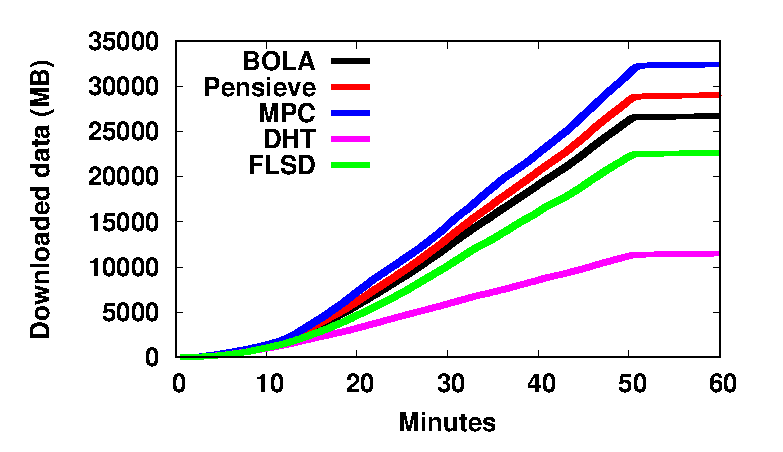
\includegraphics[width=0.49\linewidth]{img/grpbasic/cdnupload_1}
		}
		\subfloat[\label{fig:cdnuploaded_cnt} \# of segment downloads from the server]{
			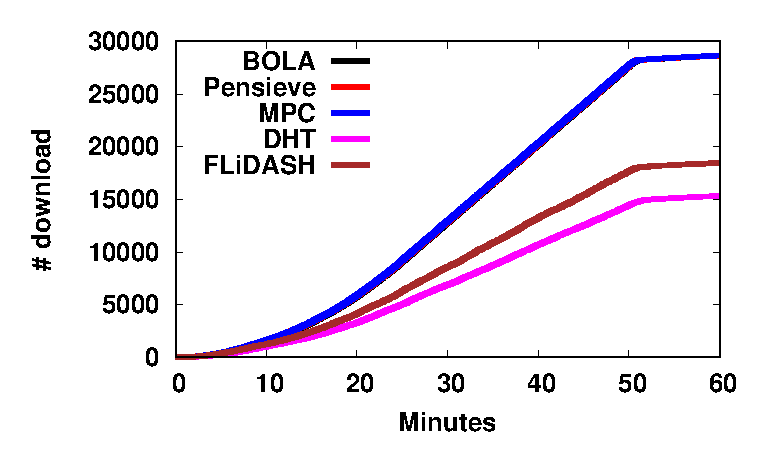
\includegraphics[width=0.49\linewidth]{img/grpbasic/cdnuploadcnt_1}
		}
	\end{center}
	\caption{\label{fig:cdnuploaded}Streaming Server Usages}
\end{figure}

One of the major objectives of \textit{CaliDASH} is to reduce the usage of streaming server when multiple co-located streaming players play the same live video. In Fig.~\ref{fig:cdnuploaded}, we plot the streaming server usage by different baselines in terms of the total bytes downloaded from the streaming server and the number of video segments directly downloaded from the streaming server. We observe that that the streaming server usages by DHT is lowest. In the case of CoaliDASH, players are bounded to receive data from its group only, while in case of DHT, a player can share segments with as many players as possible. The standalone players need to download all the segments directly from the server. Therefore, we observe a performance trade-off here -- \textit{CoaliDASH} significantly improves the QoE performance while having little increase in the streaming server load. In a nutshell, the proposed approach makes a balance between the QoE and streaming server load during the peer-assisted live video streaming.  


%Fig.~\ref{fig:avgBitrate}, \ref{fig:avgBitrateVar}, \ref{fig:Stall_Time} and \ref{fig:QoE} we report the general result we found from our experiment. Fig.~\ref{fig:QoE} is a plot of Quality of Experience. We calculate QoE using the Equation~\ref{eqn:QoE}. In the equation, $\alpha$ is the quality factor and $\beta$ and $\gamma$ are smoothness penalty and stall penalty.
%
%
%
%According to Fig.\ref{fig:avgBitrate} performance of BOLA very low and most of the players played in lower quality. BOLA is very conservative about the bitrate and very much concerned about the rebuffering time. Pensieve and MPC improved the video quality compared to the BOLA by utilising reinforcement learning and deep inspection respectively. DHT is the first system which uses the knowledge of existing players in the network. So, it improves an average video quality compared to ABR. However, CoaliDASH clustered the players and played video in sync. In Fig.~\ref{fig:avgBitratecmf}, it is clear that there are clusters of players who played video in almost equal quality. Average variation in video quality is higher for CoaliDASH. However, it is higher because it played in the video in high quality. A slight change in the quality incurs high variation.


%\begin{figure}[h]
%\captionsetup[subfigure]{}
%\begin{center}
%	\subfloat[\label{fig:benfit_bitrate} Benefit in terms of average bitrate]{
%		\includegraphics[width=0.49\linewidth]{img/grpbasic/benefit_bitrate_box_1}
%	}
%	\subfloat[\label{fig:benefit_qoe} Benefit in terms of QoE]{
%		\includegraphics[width=0.49\linewidth]{img/grpbasic/benefit_qoe_box_1}
%	}
%\end{center}
%\caption{\label{fig:benefit}Per player benefit of using CoaliDASH}
%\end{figure}



\begin{figure*}[h]
	\captionsetup[subfigure]{}
	\begin{center}
		\subfloat[\label{fig:grp_qoe}Overall QoE]{
			\includegraphics[width=0.33\linewidth]{img/grpbasic/grpsz_qoe}
		}
		\subfloat[\label{fig:grp_download}Amount of Data Upload and Download]{
			\includegraphics[width=0.33\linewidth]{img/grpbasic/grpsz_upload_download}
		}
       	\subfloat[\label{fig:grp_fairness}Fairness]{
       			\includegraphics[width=0.33\linewidth]{img/grpbasic/grpsz_fairness}
       		}
	\end{center}
	\caption{\label{fig:grpsz}Effect of Coalition Size}
\end{figure*}





%\subsection{Benefit of using CoaliDASH}
%In Fig.~\ref{fig:benefit}, we report the benefit of using CoaliDASH instead of another streaming system for each player in the system. Here we plot only two metrics, i.e. average bitrate and QoE. To measure the benefit of using CoaliDASH we need to keep the environment (i.e. network condition) of a player same for each ABR and reference network. It is possible for because our environment is simulated and the entire simulation state depends on the initial random variable\footnote{We use pseudo-random variable available in {\tt python numpy} library. It generates the same sequence of random numbers for the same seed/initial state.} state. However, it means that every time we run the experiment with the same environment, ABR and reference network, we get the same result. For this reason, we do not run the same experiment with the same environment, ABR and network. However, to measure the benefit of using CoaliDASH instead of other ABR, we run an experiment on a large set of environments and reference network. We use Equation~\ref{eqn:benefit} to compute the benefit of a single player. Here $G_g$ is the metric for using CoaliDASH and $G_o$ is the same metric for other ABR. We plot all the benefit as a box plot. Here benefit $Ben(S)==0$ means CoaliDASH performed precisely the same as the other ABR. The positive and negative benefit means the better or worse performance of CoaliDASH compared to other ABR.
%\begin{equation}
%Ben(S) = \frac{G_g - G_o}{|G_o|}
%\label{eqn:benefit}
%\end{equation}
%From Fig.~\ref{fig:benefit}, we can see that most of the player in the experiments gain some forms of benefit in terms of average playback quality as well as the QoE. The slight degradation in the benefit in terms of QoE with compared to BOLA. We have already seen in the Fig.\ref{fig:QoE} that QoE of BOLA is very high although the average quality is low because of its very low stall time. However, the overall performance of CoaliDASH is higher than any other existing ABR or systems.
%\subsection{Effect of group size}
In all the previous experiments, we have fixed the maximum coalition size to 4 players. Here we check the effect of the increasing the coalition size. Fig.~\ref{fig:grp_qoe} and Fig.~\ref{fig:grp_download} shows the impact of different coalition sizes on the overall QOE and the total amount of data downloaded from the streaming server, respectively. We observe that a large coalition size provides better QoE because it gives more time to download a segment. However, in the case of a large coalition, every player has to upload more data to the other members of the coalition, which incurs an additional overhead.

%\subsection{Fairness}
In collaborative scenario, fairness among the members is an important metric. In our evaluation, we measure the fairness among the coalition members using Jain fairness index on QoE among the players \cite{jain1999throughput}. We measure the fairness among players in two categories, i) intra-coalition fairness (fairness among the coalition members of a coalition) and ii)inter-coalition fairness (fairness among the coalitions). The results are reported in Fig.~\ref{fig:grp_fairness}. We have computed fairness for seven different coalition sizes. Here we observe that the intra-coalition fairness index is always close to 1, which indicates a perfect fairness. However, inter-coalition fairness is not very high. It is expected as different coalitions can play video in different video quality which has a major contribution to the overall QoE. 
%From this result, we can conclude that CoaliDASH is fair.

%
%\subsection{Takeways of the study}
\label{chap03s1:sec:conclusion}

In this work, we studied the internal working of YouTube's bitrate adaptation algorithm, by identifying important parameters and exploring their roles.
We can summarize the outcomes and contributions of our work as follows.
%We observed that YouTube adapts segment length in addition to quality level, a behavior not been reported earlier.
%As an implication, we observed that data wastage for a playback session is significantly lower than estimated previously.
%We further provided an analytical model, augmented with a machine learning based classifier, to predict data consumption in adavance for a video playback session.
%As an immediate future direction, we would like to explore other important implications of segment length adaption for YouTube.

{\bf Experimental observations:} Our experiments reinforce the earlier reported observation that video quality adaptation is based on buffer size distribution at the YouTube client.
However, we also observe that when encountered with a drop in network bandwidth, YouTube makes an effort to adaptively change segment lengths of the downloaded video chunks, before downgrading video quality -- this observation, to the best of our knowledge, has not been reported in any prior work.
In fact, we find that YouTube employs an opportunistic approach of joint video quality and streaming rate adaptation, which is similar to the elastic behavior characteristic  observed in TCP traffic (\S\ref{chap03s1:sec:parameters}).

{\bf Data wastage during YouTube streaming:} Downloaded data can end up being wasted in adaptive bit-rate streaming when, due to a sudden improvement in network conditions, a higher quality video segment is downloaded for viewing, even when a lower quality segment for the same playback duration already exists -- the lower quality segment is rendered unproductive.
In light of our experimental observations, we ask the following research question: ``How does segment length adaptation affect data wastage in YouTube adaptive streaming?''
The question is particularly interesting, since many existing works (including~\cite{sieber2016sacrificing} recently) have studied data wastage in DASH implementations, including that of YouTube.
We experimentally determine the data wastage ratio involved in YouTube adaptive streaming to be around $0.82x10^{-6}$ on an average, which is significantly lesser than values reported by earlier studies.% (\notess{exact value from cited work}).
We reason that such overestimations in earlier works stemmed from their incorrect assumption that the segment size remains constant, which led to gross approximations in their data wastage computations.

{\bf Model to predict data consumption:} Furthermore, we realize that prediction of data consumption (both productive and wasted) even before a video has actually played, can serve as an important parameter for more intelligent streaming in challenging scenarios.
Suppose an user is traveling through a zone of irregular connectivity, thereby resulting in fluctuating bandwidth. It can be noted that existing mechanisms, such as~\cite{Zou2015} and the references therein, can predict the bandwidth fluctuation pattern a priori under many mobility patterns such as predicted urban mobility.  
The user would ideally wish to watch videos for as long as possible, without sacrificing her quality of experience too much (streaming in lowest available resolution is too extreme for her). 
Assuming the YouTube client has prior information of these challenges, and can predict data consumption, it can decide upon the most balanced quality level to start streaming in, so that the data download is minimized.
To such ends, we propose an analytical model, augmented with a machine learning based classifier, using which one can estimate data consumption even before actually playing a YouTube video, if channel conditions and the initial video quality level are known.

{\bf Contributions:} In summary, our contributions in this work are:
\begin{enumerate}
	\item We illustrate a methodology to study YouTube's adaptive streaming behavior in-depth (\S\ref{chap03s1:sec:experiments}) -- we identify and closely study the interplay among important parameters enabling this streaming algorithm (\S\ref{chap03s1:sec:parameters}).
	\item Our experiments reveal that YouTube adapts the {\it segment length} parameter before attempting to adapt video resolution -- a phenomenon not reported in the literature (\S\ref{chap03s1:subsec:seglength}).
	\item We observe that segment length adaptation leads to much lower values of data wastage on average, than reported by prior studies.
	\item We propose an analytical model, augmented with a machine learning based classifier, which enables prediction of data consumption for an initial playback video quality when it is possible to estimate the network conditions a priori using existing mechanism like~\cite{Zou2015}  (\S\ref{chap03s1:sec:model}).
\end{enumerate}



\singlespacing
\small
\bibliographystyle{IEEEtran}
\bibliography{ref/references} 
%

\end{document}
